% SayNote - Chapitre II: Planification et Conception UX
% Ce chapitre présente la planification du projet et la conception de l'expérience utilisateur

% --- Introduction non numérotée ---
\begin{center}
    \textbf{\large Introduction du Chapitre}
    \end{center}
    
        Ce chapitre présente la démarche de planification et la conception de l'expérience utilisateur (UX) pour SayNote. Il détaille la méthodologie adoptée, la structuration du projet, ainsi que l'approche centrée sur l'utilisateur, en mettant l'accent sur l'importance des diagrammes UML et techniques pour la modélisation du système. Le lecteur découvrira comment la planification et la conception UX préparent le terrain pour une implémentation efficace et cohérente.
    
    \section{Introduction}
    
    Après avoir identifié les problématiques et défini le concept de SayNote dans le chapitre précédent, nous nous concentrons maintenant sur la planification du projet et la conception de l'expérience utilisateur. Cette phase est cruciale pour transformer notre vision en un plan d'action concret et en une interface utilisateur intuitive qui répond aux besoins réels des utilisateurs.
    
    La planification et la conception UX sont particulièrement importantes pour SayNote en raison de son approche novatrice combinant commandes vocales et édition par blocs. L'interaction vocale, bien que naturelle pour la communication humaine, présente des défis uniques lorsqu'elle est appliquée au contrôle d'une interface numérique. Notre objectif est de créer une expérience fluide et intuitive qui tire pleinement parti des capacités vocales tout en offrant une interface visuelle cohérente et familière.
    
    Ce chapitre détaille notre méthodologie de planification, notre approche de l'expérience utilisateur basée sur la recherche et l'empathie, ainsi que la conception technique du système d'information qui sous-tend l'application.
    
    \section{Planification du projet}
    
    \subsection{Méthodologie de planification}
    
    Pour le développement de SayNote, nous avons adopté une approche agile, plus précisément la méthodologie Scrum, complétée par des éléments de Design Thinking pour la conception UX. Cette combinaison nous permet d'itérer rapidement tout en gardant l'utilisateur au centre de notre processus de conception.
    
    \subsubsection{Approche Agile Scrum}
    
    L'approche Scrum a été choisie pour sa flexibilité et sa capacité à s'adapter aux changements inhérents au développement d'un produit innovant comme SayNote. Nous avons organisé notre travail en sprints de deux semaines, chacun comportant les événements standards de Scrum:
    
    \begin{itemize}
        \item \textbf{Sprint Planning:} Au début de chaque sprint, l'équipe sélectionne les tâches du Product Backlog à réaliser, en se basant sur leur priorité et la capacité de l'équipe.
        
        \item \textbf{Daily Stand-up:} Réunions quotidiennes de 15 minutes pour synchroniser les activités et identifier les obstacles.
        
        \item \textbf{Sprint Review:} À la fin de chaque sprint, l'équipe présente les fonctionnalités développées aux parties prenantes pour obtenir des retours.
        
        \item \textbf{Sprint Retrospective:} L'équipe analyse ce qui a bien fonctionné et ce qui peut être amélioré pour le prochain sprint.
    \end{itemize}
    
    Cette approche nous permet de livrer régulièrement des incréments de produit fonctionnels et d'ajuster notre direction en fonction des retours utilisateurs et des défis techniques rencontrés.
    
    \subsubsection{Design Thinking pour l'UX}
    
    En parallèle de Scrum, nous avons intégré le processus de Design Thinking pour la conception de l'expérience utilisateur, qui comprend cinq phases:
    
    \begin{enumerate}
        \item \textbf{Empathie:} Comprendre profondément les besoins, les frustrations et les aspirations des utilisateurs potentiels à travers des entretiens et des observations.
        
        \item \textbf{Définition:} Synthétiser les connaissances acquises pour définir clairement les problèmes à résoudre.
        
        \item \textbf{Idéation:} Générer un large éventail d'idées et de solutions potentielles sans contraintes initiales.
        
        \item \textbf{Prototypage:} Créer des représentations tangibles des solutions les plus prometteuses.
        
        \item \textbf{Test:} Recueillir les retours des utilisateurs sur les prototypes pour affiner et améliorer les solutions.
    \end{enumerate}
    
    Cette approche centrée sur l'utilisateur est particulièrement pertinente pour SayNote, où l'interaction vocale nécessite une compréhension fine des attentes et des comportements des utilisateurs.
    
        
    \subsection{Planification}
    
    \subsubsection{Roadmap du projet}
    
    La roadmap de SayNote a été structurée en quatre phases principales, chacune comportant plusieurs sprints:
    
    \begin{enumerate}
        \item \textbf{Phase de recherche et de conception (2 mois):}
        \begin{itemize}
            \item Recherche utilisateur et analyse concurrentielle
            \item Définition des personas et des scénarios d'utilisation
            \item Conception de l'architecture du système
            \item Wireframing et prototypage initial
        \end{itemize}
        
        \item \textbf{Phase de développement MVP (4 mois):}
        \begin{itemize}
            \item Mise en place de l'infrastructure technique
            \item Développement du backend et de l'API
            \item Implémentation de l'éditeur de notes par blocs (avec BlockNote.js)
            \item Intégration de la reconnaissance vocale de base
            \item Développement de l'interface utilisateur mobile (Expo/React Native)
        \end{itemize}
        
        \item \textbf{Phase d'amélioration et d'expansion (3 mois):}
        \begin{itemize}
            \item Optimisation des algorithmes de traitement du langage naturel
            \item Expansion des commandes vocales supportées
            \item Développement de l'interface web
            \item Implémentation des fonctionnalités de sous-pages et de hiérarchie de notes
        \end{itemize}
        
        \item \textbf{Phase de finalisation et de lancement (1 mois):}
        \begin{itemize}
            \item Tests utilisateurs approfondis
            \item Correction des bugs et optimisations finales
            \item Préparation du matériel marketing
            \item Lancement officiel de l'application
        \end{itemize}
    \end{enumerate}
    
    % Explication brève avant chaque figure
        \begin{figure}[htbp]
        \centering
        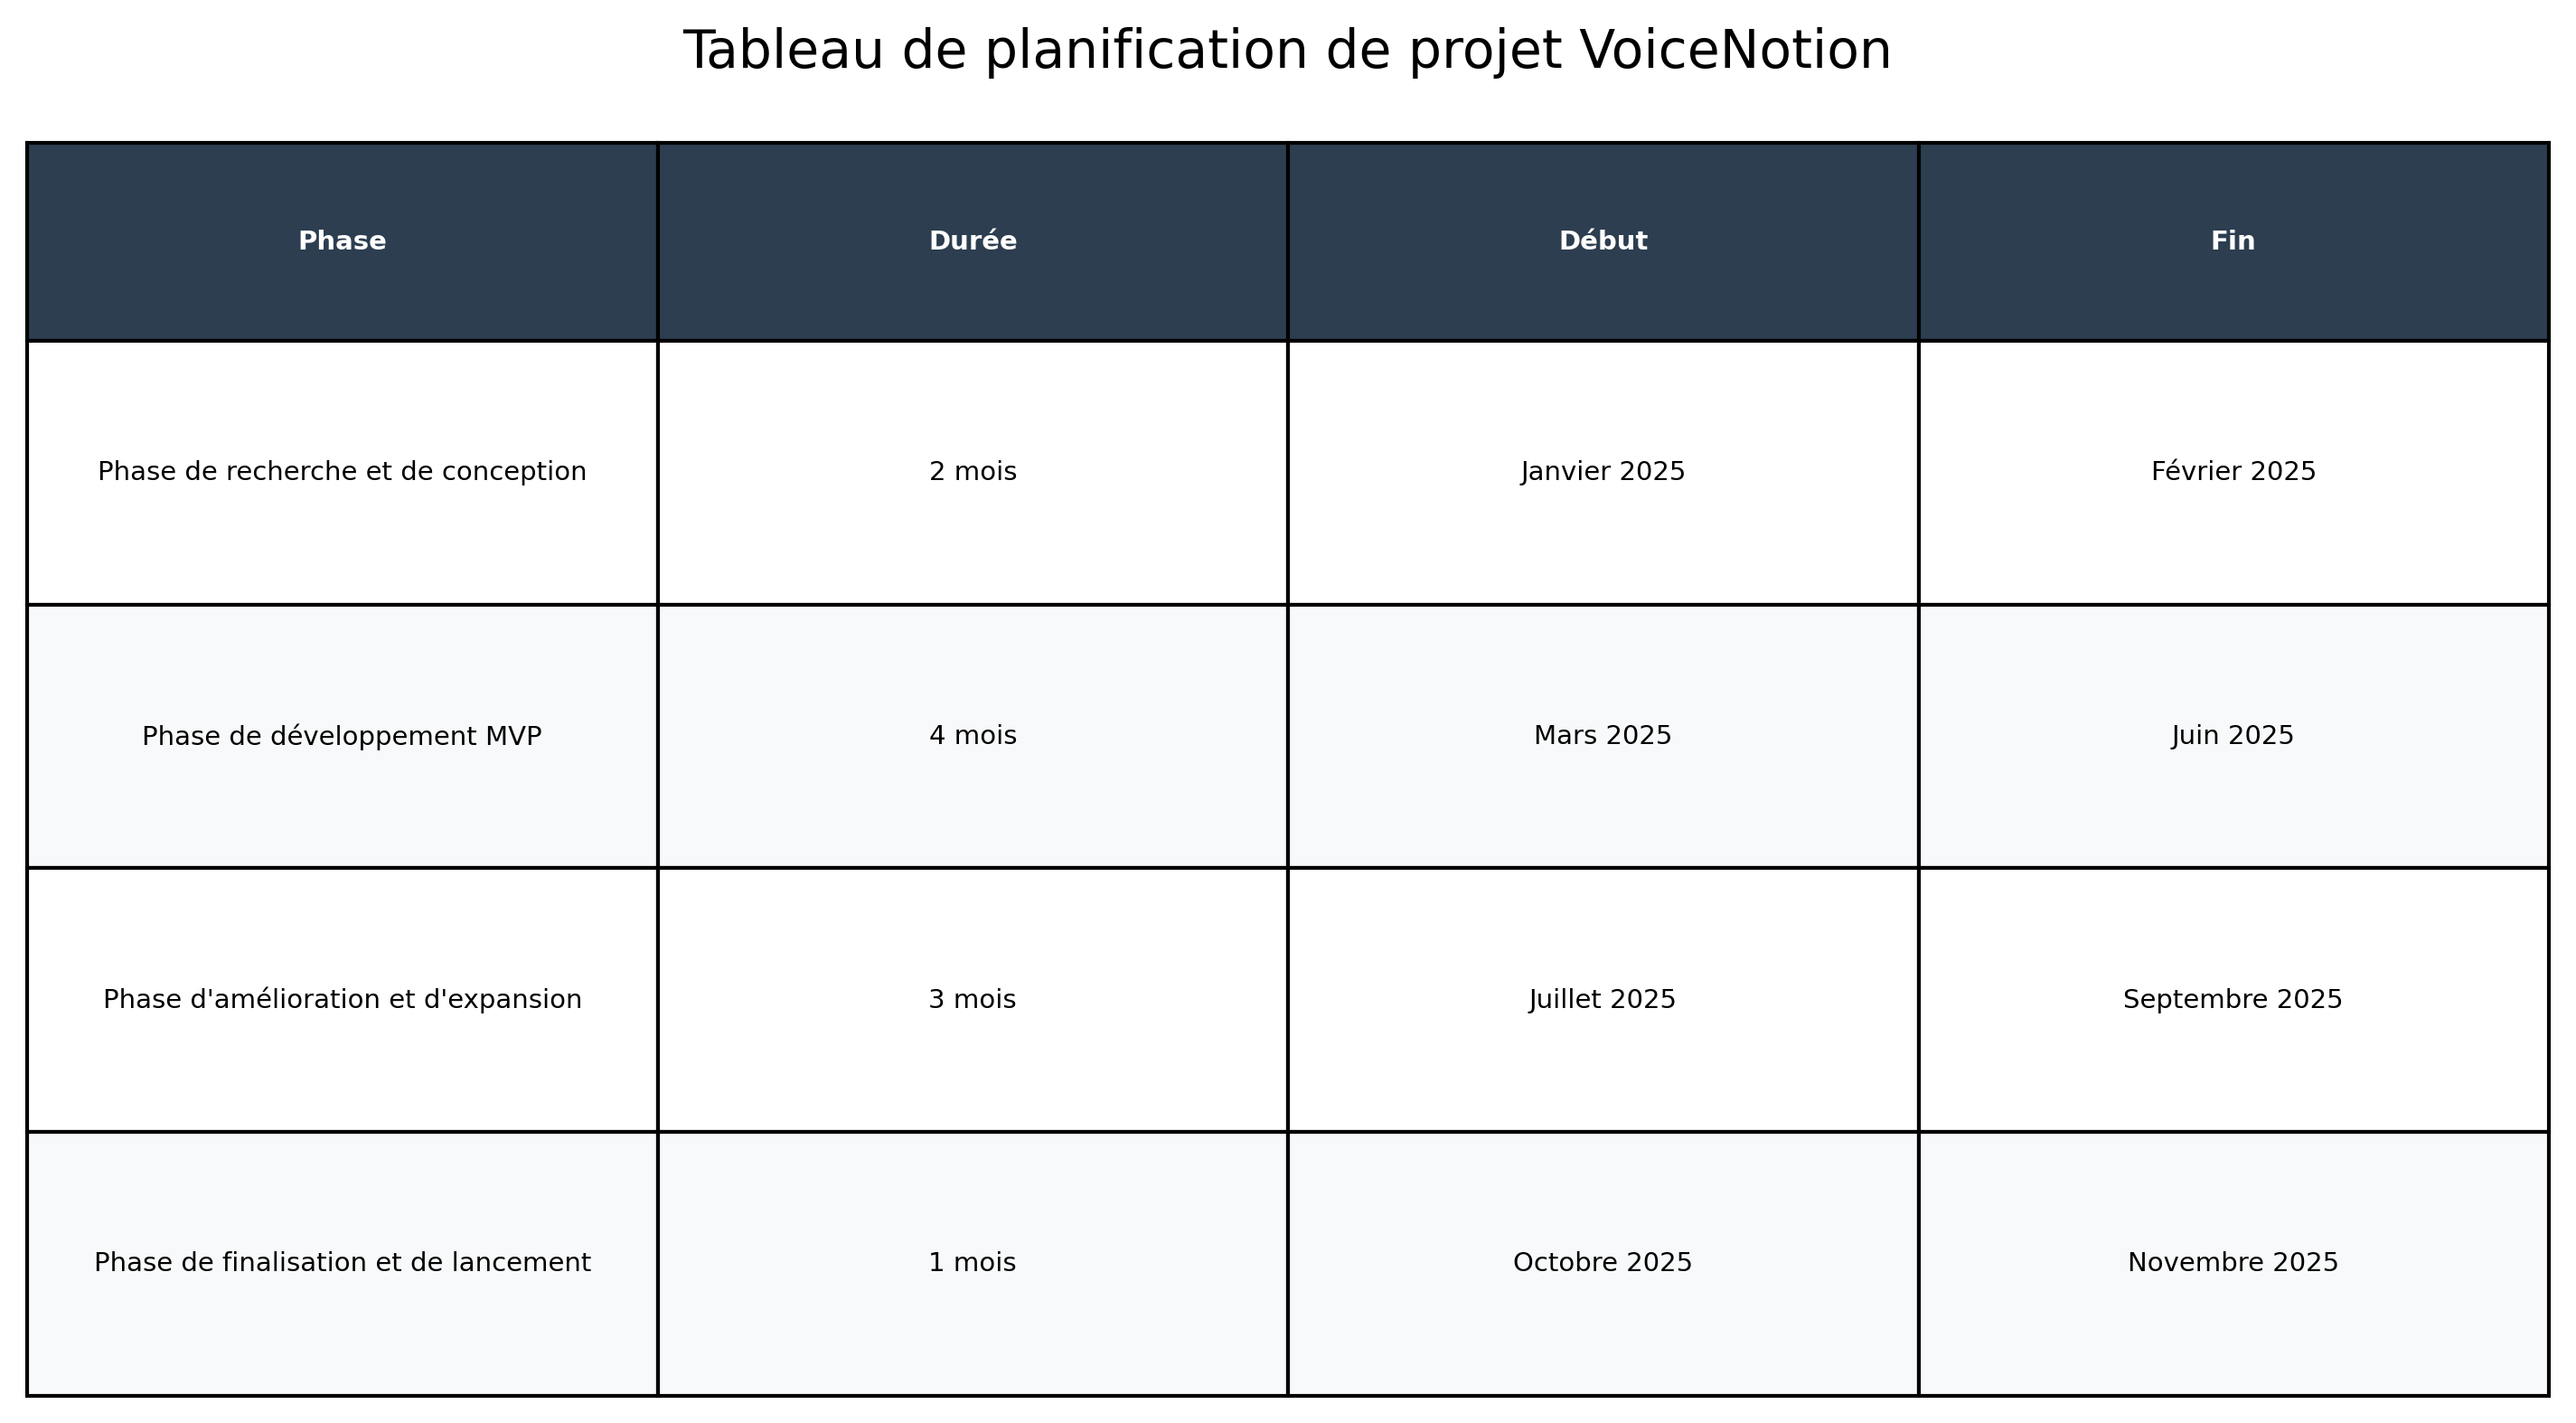
\includegraphics[width=0.9\textwidth]{assets/docs/planification_table.png}
        \caption{Tableau de planification de projet}
        \label{fig:planification_table}
    \end{figure}
    
    % Explication brève avant chaque figure
        \begin{figure}[htbp]
        \centering
        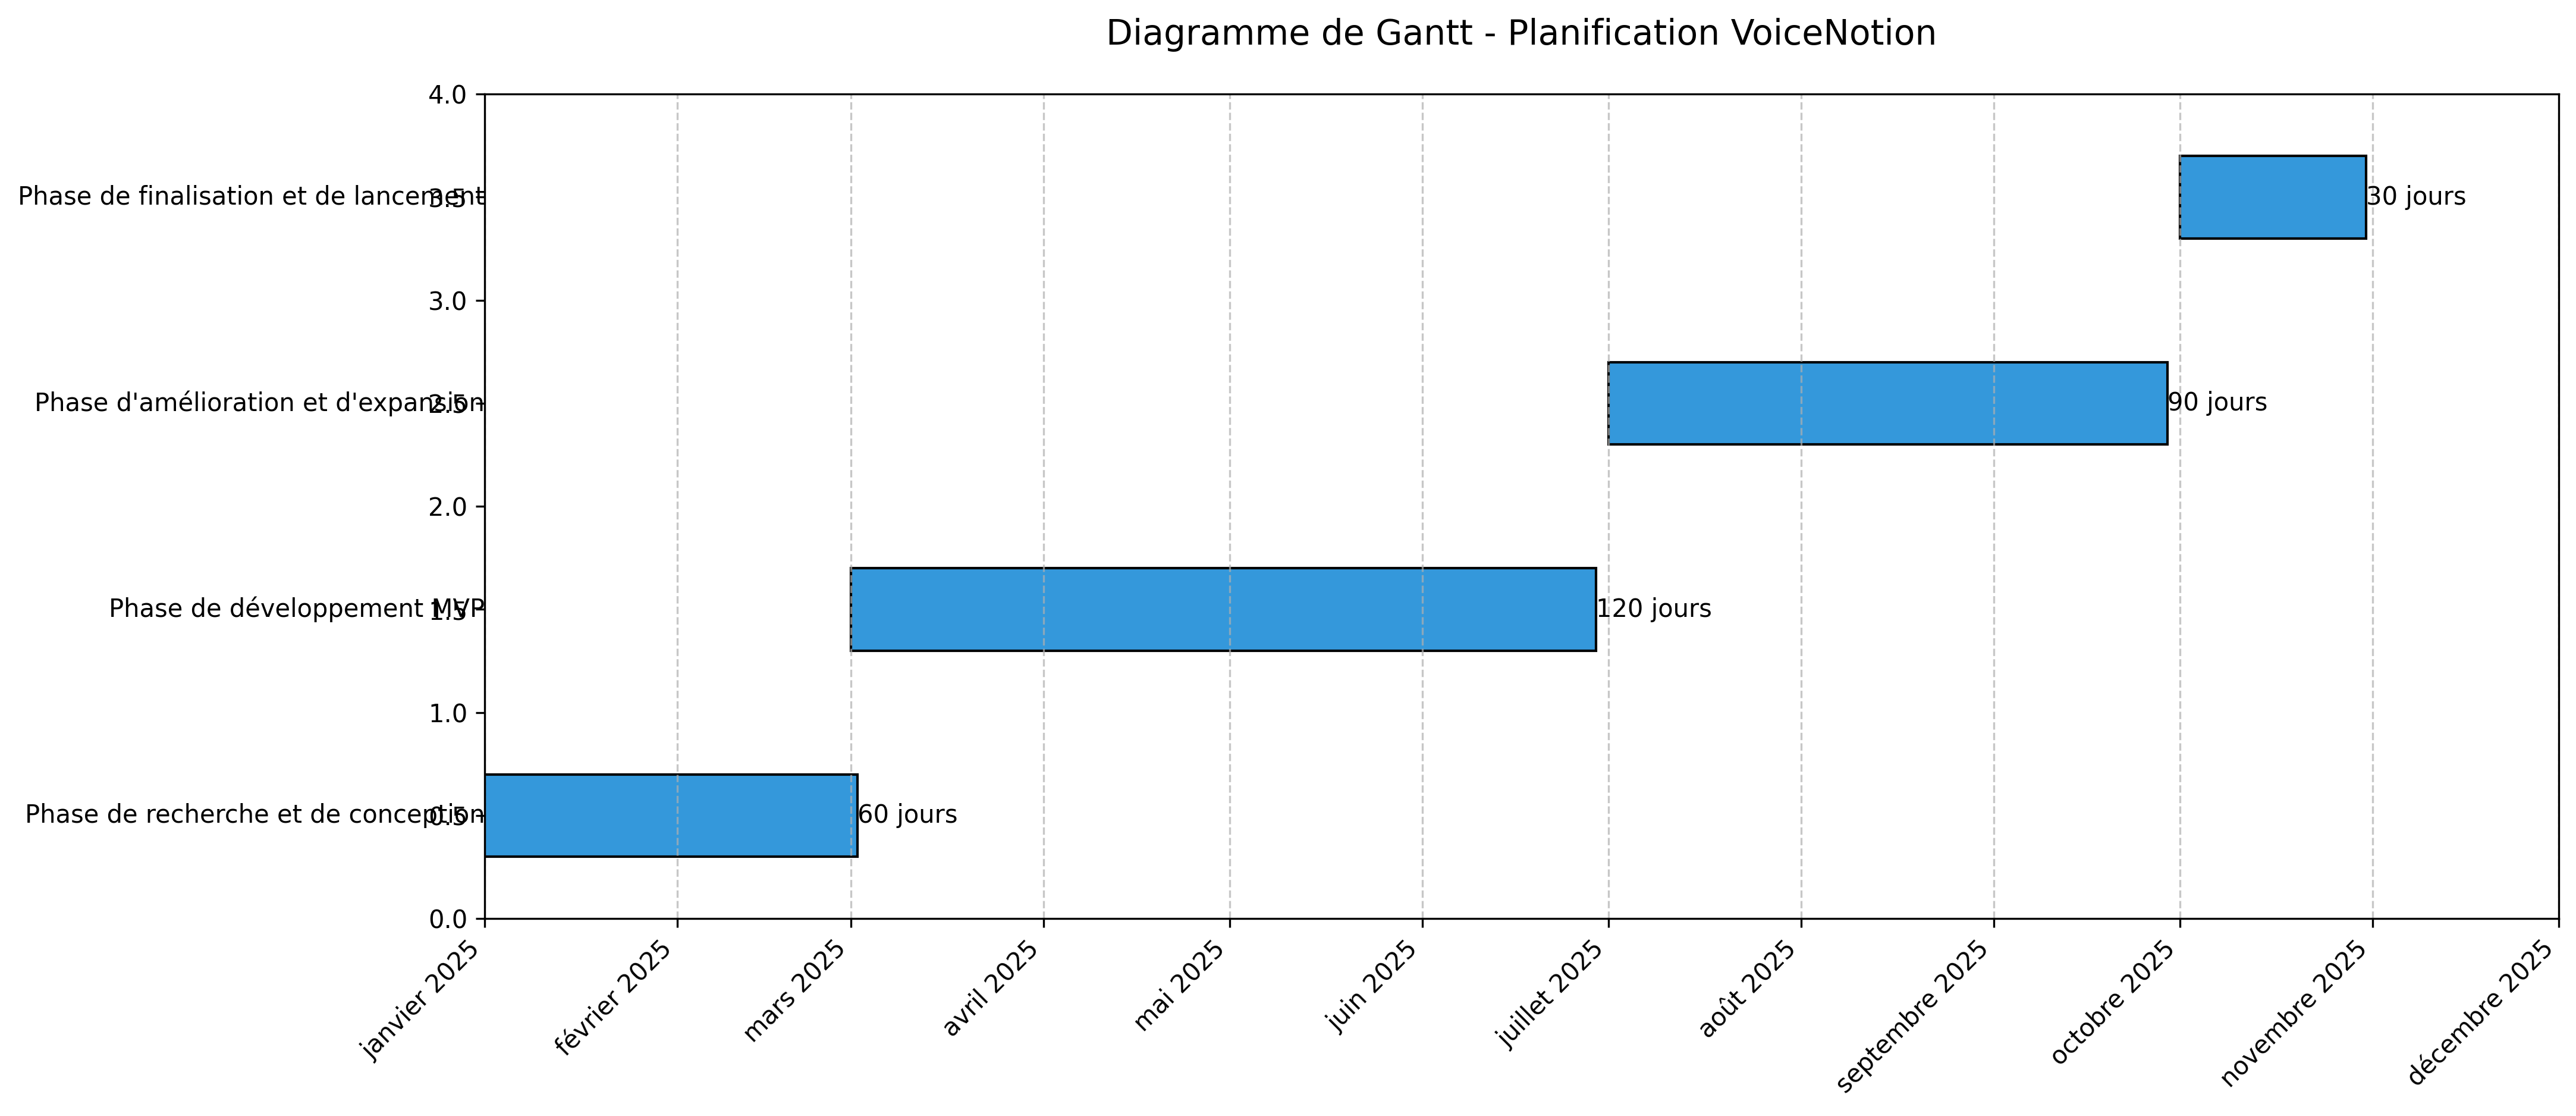
\includegraphics[width=0.9\textwidth]{assets/docs/gantt_chart.png}
        \caption{Diagramme de Gantt de planification de projet}
        \label{fig:gantt_chart}
    \end{figure}
    
    \paragraph{Calendrier détaillé (avril–juin 2025)}
Le tableau~\ref{fig:planification_table} fournit un aperçu visuel ; ci-dessous figure le même planning avec les dates exactes :

\begin{itemize}
  \item \textbf{Recherche \& planification} : 01/04/2025 – 07/04/2025
  \item \textbf{Conception graphique} : 08/04/2025 – 22/04/2025
    \begin{itemize}
      \item \textit{UI/UX Design} : 23/04/2025 – 30/04/2025
      \item \textit{Design System} : 23/04/2025 – 25/04/2025
      \item \textit{Prototypage} : 26/04/2025 – 28/04/2025
      \item \textit{Wireframing} : 29/04/2025 – 30/04/2025
      \item \textit{Animation vidéo} : 01/05/2025 – 03/05/2025
    \end{itemize}
  \item \textbf{Architecture système} : 04/05/2025 – 07/05/2025
    \begin{itemize}
      \item \textit{Conception base de données} : 08/05/2025 – 10/05/2025
    \end{itemize}
  \item \textbf{Développement \& build} : 11/05/2025 – 10/06/2025
    \begin{itemize}
      \item \textit{API (Back-End)} : 11/05/2025 – 24/05/2025
      \item \textit{Site client (Web)} : 11/05/2025 – 31/05/2025
      \item \textit{Application mobile} : 11/05/2025 – 31/05/2025
      \item \textit{Hébergement \& déploiement} : 01/06/2025 – 05/06/2025
      \item \textit{Tests} : 06/06/2025 – 10/06/2025
    \end{itemize}
  \item \textbf{Synthèse et documentation} : 11/06/2025 – 20/06/2025
    \begin{itemize}
      \item \textit{Rapport de projet} : 13/06/2025 – 17/06/2025
      \item \textit{Présentation} : 18/06/2025 – 20/06/2025
    \end{itemize}
\end{itemize}

\subsubsection{Gestion des risques}
    
    Nous avons identifié plusieurs risques potentiels pour le projet et élaboré des stratégies d'atténuation:
    
    \begin{table}[H]
    \centering
    \begin{tabular}{|p{3cm}|p{5cm}|p{5cm}|}
    \hline
    \textbf{Risque} & \textbf{Impact potentiel} & \textbf{Stratégie d'atténuation} \\
    \hline
    Précision limitée de la reconnaissance vocale & Frustration utilisateur, abandon de l'application & Implémentation d'un mécanisme de correction, modes d'entrée alternatifs, tests extensifs avec différents accents \\
    \hline
    Complexité technique de l'intégration BlockNote & Retards de développement, problèmes de performance & Spike techniques précoces, exploration des alternatives, recrutement d'expertise spécifique \\
    \hline
    Expérience utilisateur non intuitive & Courbe d'apprentissage abrupte, faible adoption & Tests utilisateurs fréquents, approche itérative, tutoriels intégrés \\
    \hline
    Limites des API Gemini & Fonctionnalités restreintes, dépendance à un tiers & Plan de secours avec solutions alternatives, découplage de l'architecture \\
    \hline
    Problèmes de performance sur appareils mobiles & Lenteur, consommation excessive de batterie & Optimisation continue, tests sur différents appareils, métriques de performance \\
    \hline
    \end{tabular}
    \caption{Tableau des risques et stratégies d'atténuation}
    \label{tab:risk_management}
    \end{table}
    
    \section{Expérience d'utilisateur (UX)}
    
    \subsection{Recherche}
    
    La conception de SayNote est fondée sur une recherche approfondie pour comprendre les besoins, les attentes et les points de friction des utilisateurs potentiels en matière de prise de notes.
    
    \subsubsection{Méthodologie de recherche}
    
    Notre recherche a combiné plusieurs approches:
    
    \begin{itemize}
        \item \textbf{Entretiens qualitatifs:} Nous avons mené 15 entretiens approfondis avec des utilisateurs potentiels issus de nos groupes cibles (étudiants, professionnels, créateurs de contenu).
        
        \item \textbf{Analyse concurrentielle:} Étude détaillée des applications existantes (Notion, Evernote, OneNote, Google Keep) pour identifier les forces, les faiblesses et les opportunités d'innovation.
        
        \item \textbf{Sondage en ligne:} Un questionnaire distribué à 50 participants pour quantifier les préférences et les habitudes de prise de notes.
        
        \item \textbf{Sessions d'observation:} Observation de 8 utilisateurs dans leur environnement naturel pendant qu'ils prenaient des notes, révélant des comportements et des défis non exprimés lors des entretiens.
    \end{itemize}
    
    \subsubsection{Principaux insights}
    
    Cette recherche a mis en lumière plusieurs insights clés qui ont guidé notre conception:
    
    \begin{enumerate}
        \item 78\% des participants trouvent que la saisie manuelle limite leur capacité à capturer rapidement les informations lors de réunions ou de conférences.
        
        \item Les utilisateurs de Notion apprécient la flexibilité de la structure par blocs, mais 65\% trouvent la courbe d'apprentissage trop abrupte.
        
        \item 92\% des participants ont exprimé de l'intérêt pour les commandes vocales, mais 71\% craignent qu'elles ne soient pas assez précises ou intuitives.
        
        \item Les utilisateurs mobiles (81\% de notre échantillon) prennent des notes dans des contextes variés où le clavier n'est pas toujours optimal (transports, déplacements, exercice).
        
        \item La structuration post-capture est identifiée comme l'un des plus grands défis, avec 85\% des participants qui admettent ne jamais réorganiser leurs notes brutes par manque de temps.
    \end{enumerate}
    
    % Explication brève avant chaque figure
        \begin{figure}[htbp]
        \centering
        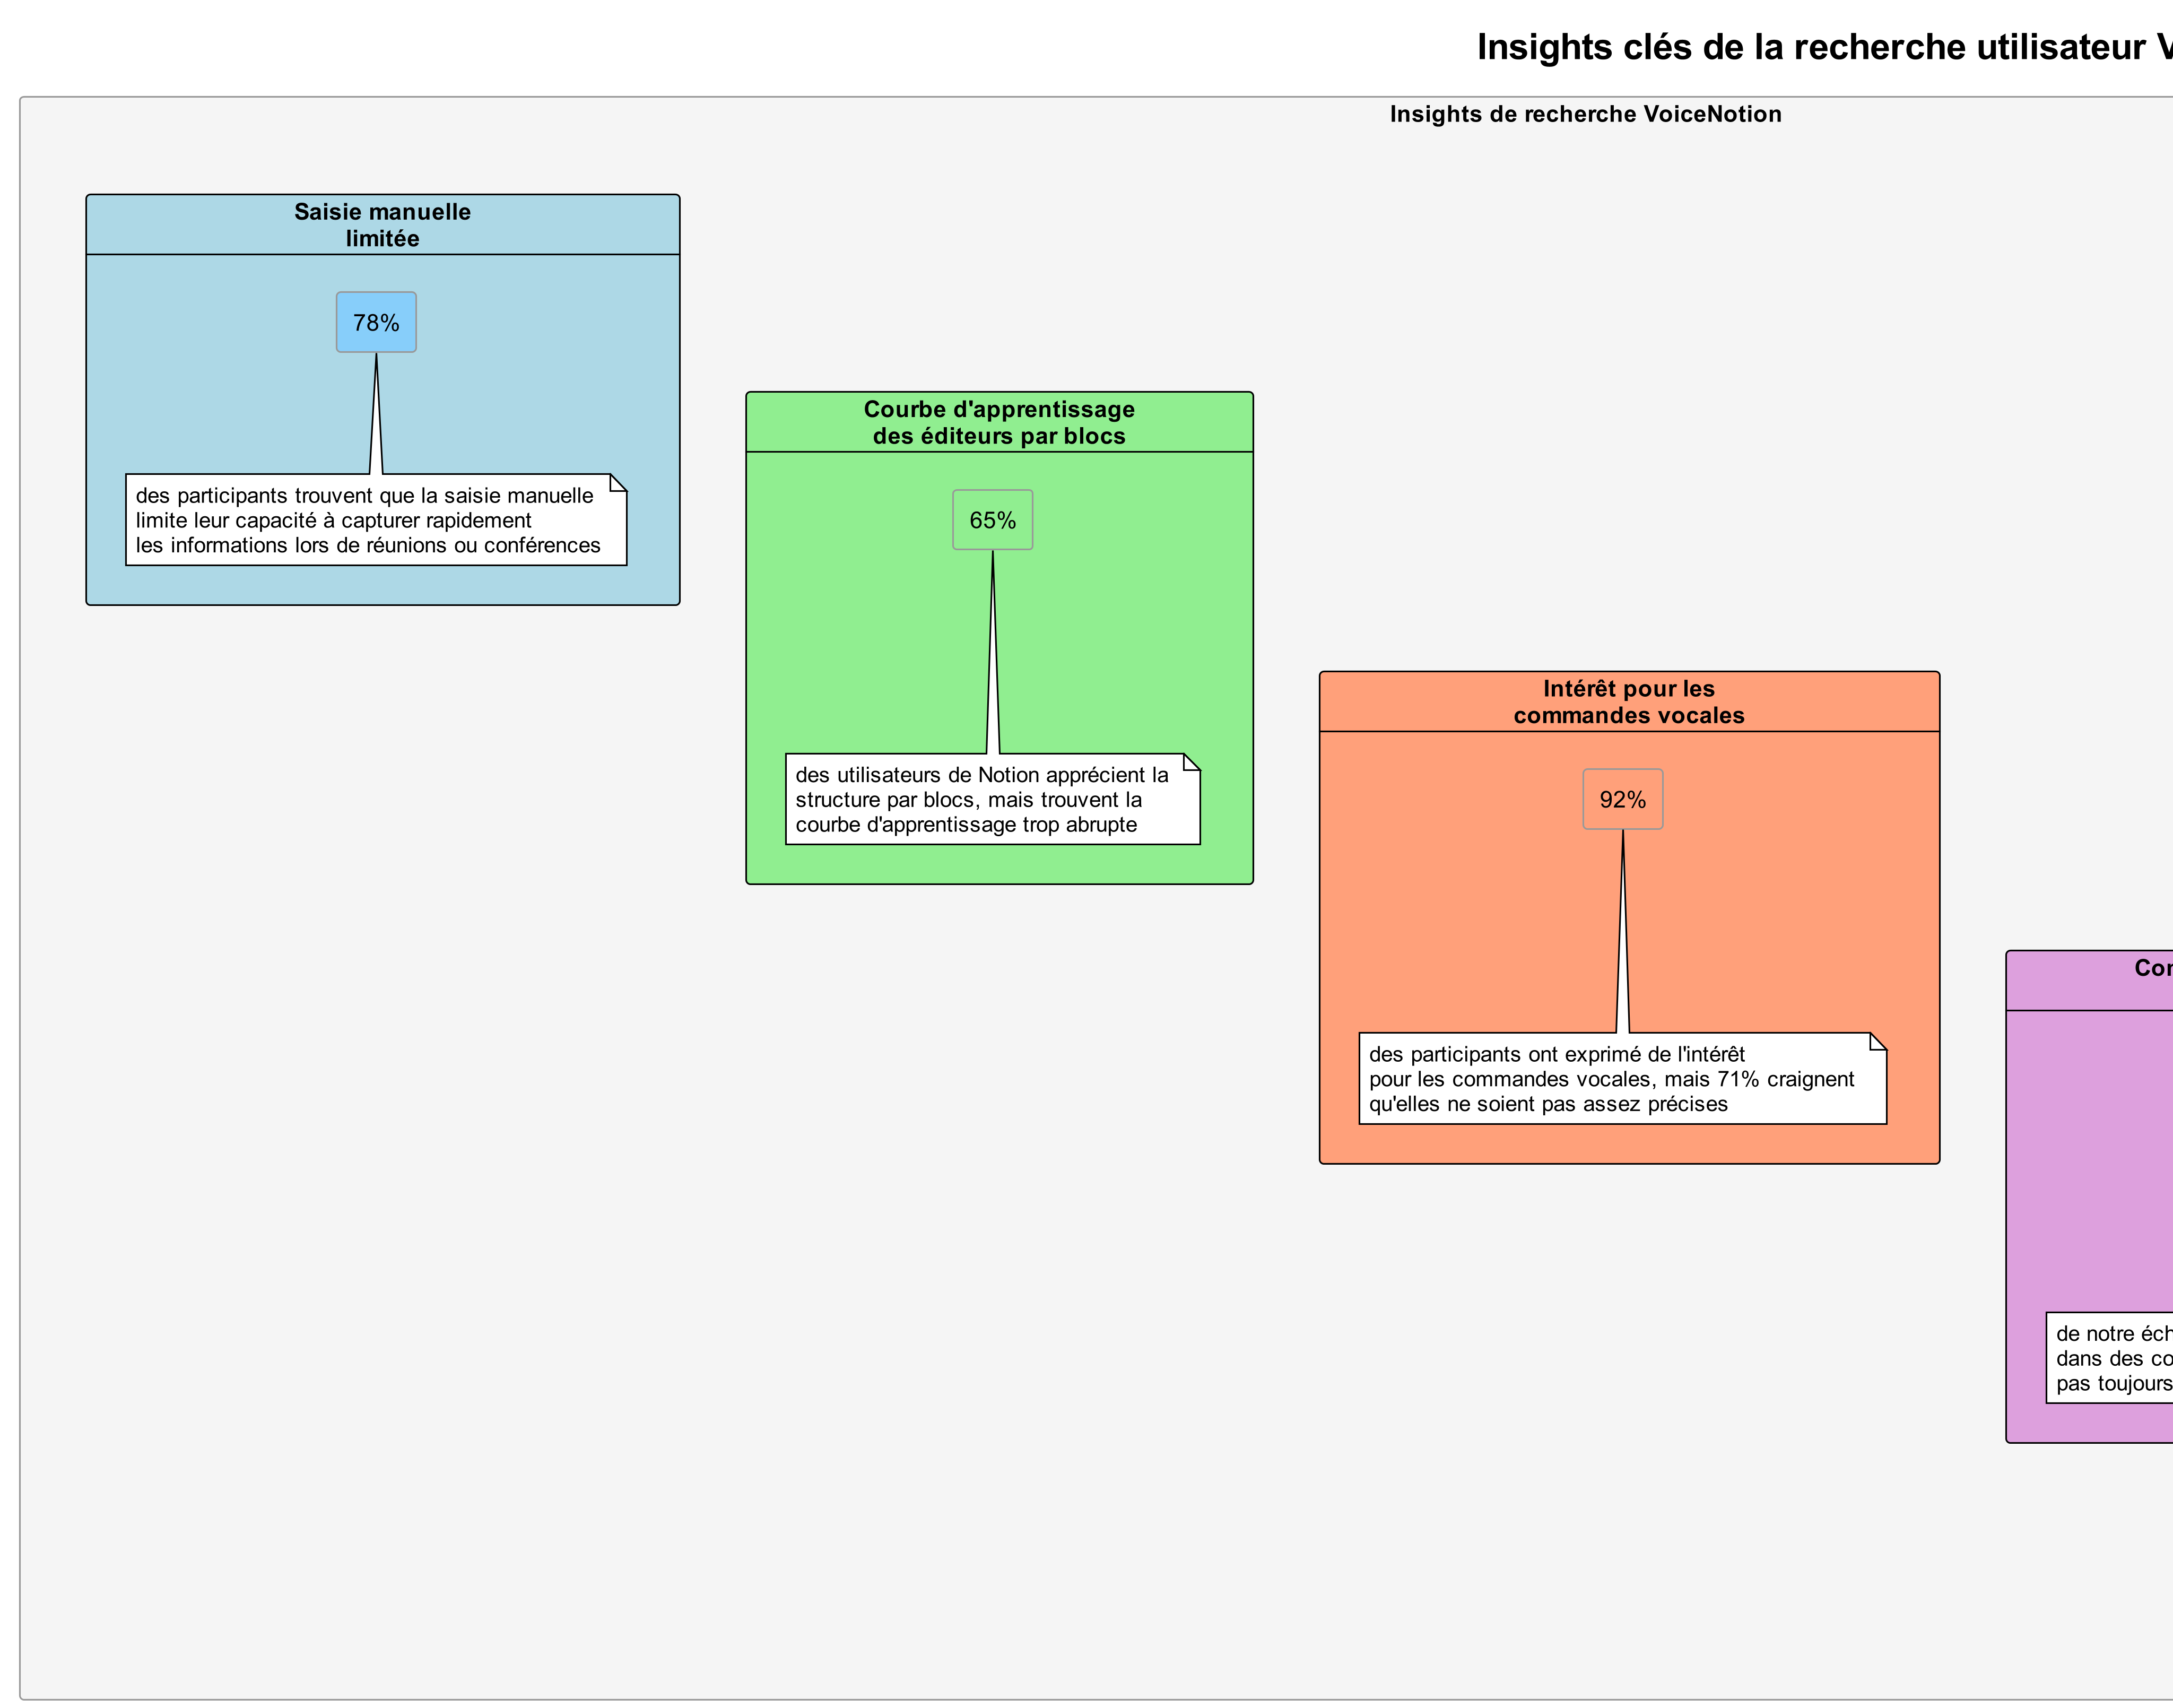
\includegraphics[width=0.75\textwidth]{assets/docs/user_research_insights.png}
        \caption{Synthèse des principaux insights de recherche utilisateur}
        \label{fig:user_research_insights}
    \end{figure}
    
    \subsection{Empathie}
    
    \subsubsection{Personas utilisateur}
    
    Basés sur notre recherche, nous avons développé deux personas principaux qui représentent nos utilisateurs cibles:
    
    \begin{figure}[H]
        \centering
        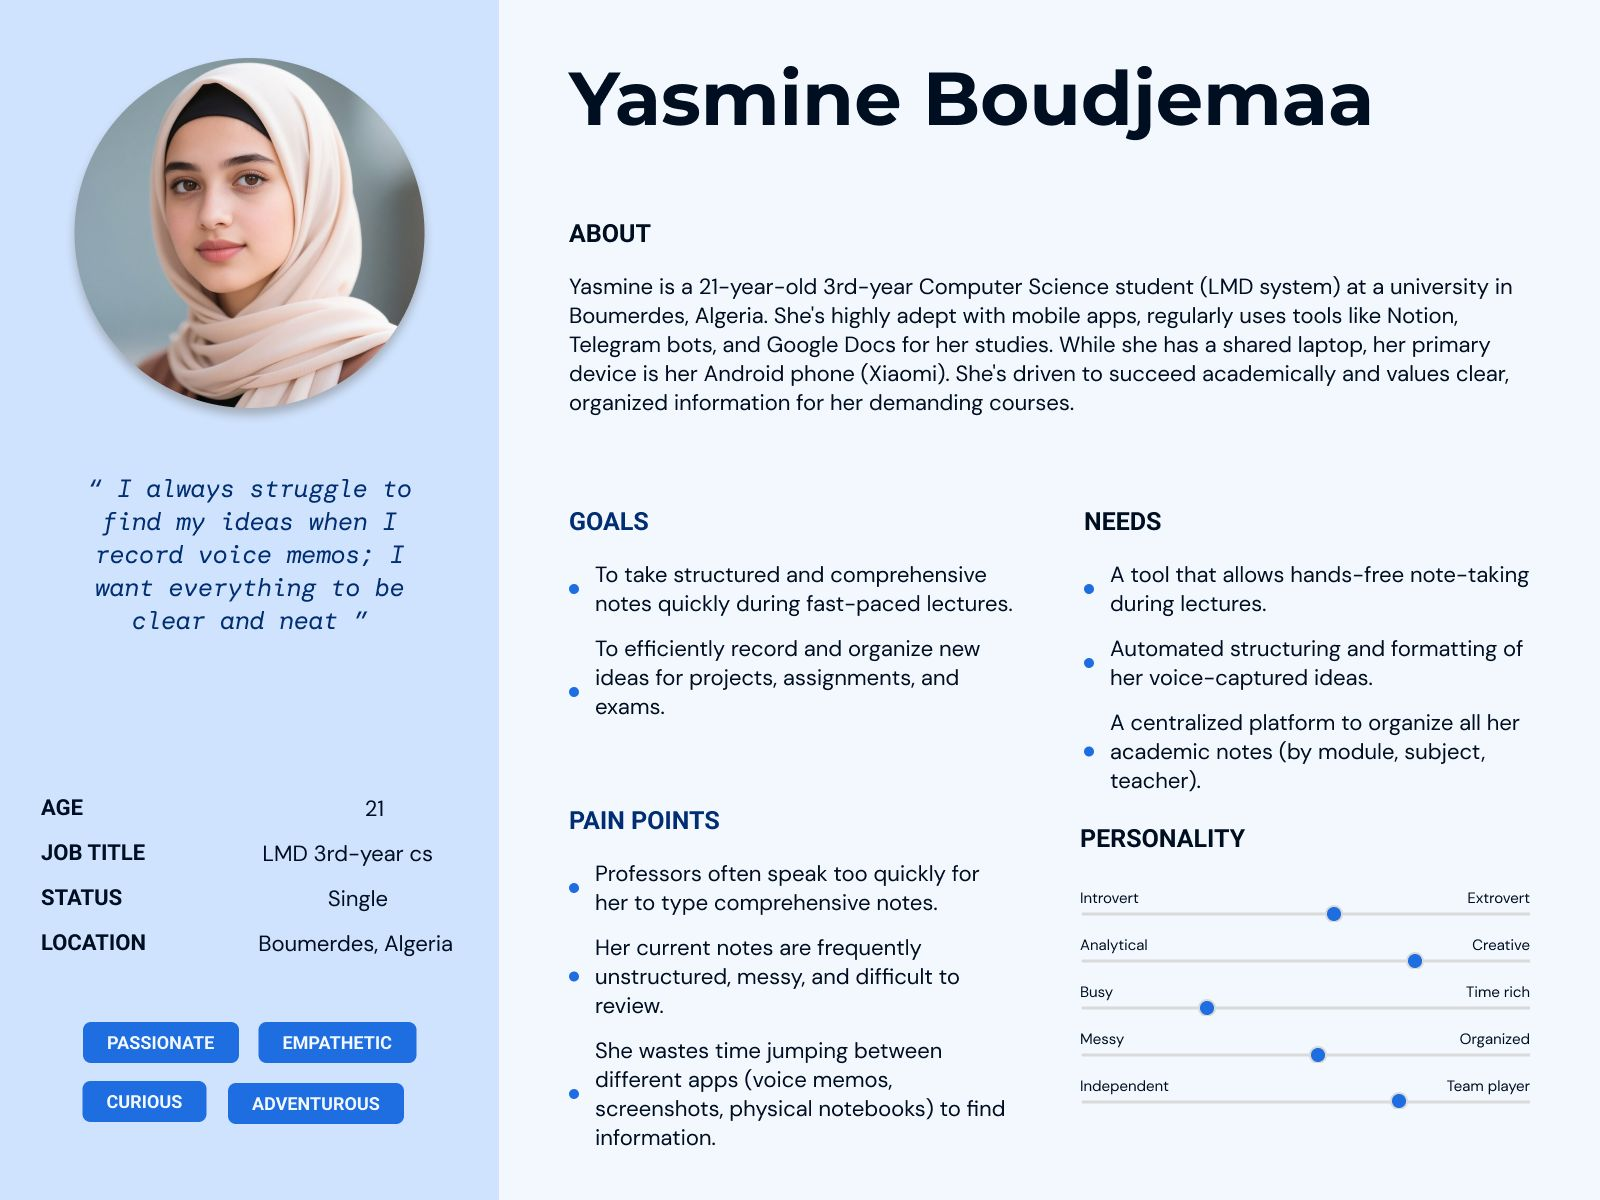
\includegraphics[width=\textwidth]{assets/docs/yassmine-personaa.jpg}
    \end{figure}
    
    \paragraph{Persona 1: Yasmine l'Étudiante en Informatique}
    
    
    \begin{itemize}
        \item \textbf{Profil:} Étudiante de 21 ans en 3ème année d'Informatique à Boumerdes. Adepte des applications mobiles (Notion, Telegram, Google Docs), elle utilise principalement son téléphone Android.
        \item \textbf{Objectifs:} Prendre des notes structurées rapidement en cours, organiser efficacement ses idées, et maintenir un système de notes propre sans réécriture manuelle.
        \item \textbf{Frustrations:} Difficulté à suivre les professeurs qui parlent vite, notes désordonnées, perte de temps entre plusieurs applications, et réorganisation manuelle fastidieuse.
        \item \textbf{Comportements:} Jongle entre mémos vocaux, captures d'écran et cahiers. Passe beaucoup de temps à réécrire et à organiser ses notes, souvent tard le soir.
        \item \textbf{Citation:} "J'ai toujours du mal à retrouver mes idées lorsque j'enregistre des mémos vocaux ; je veux que tout soit clair et bien rangé."
    \end{itemize}

    \begin{figure}[H]
        \centering
        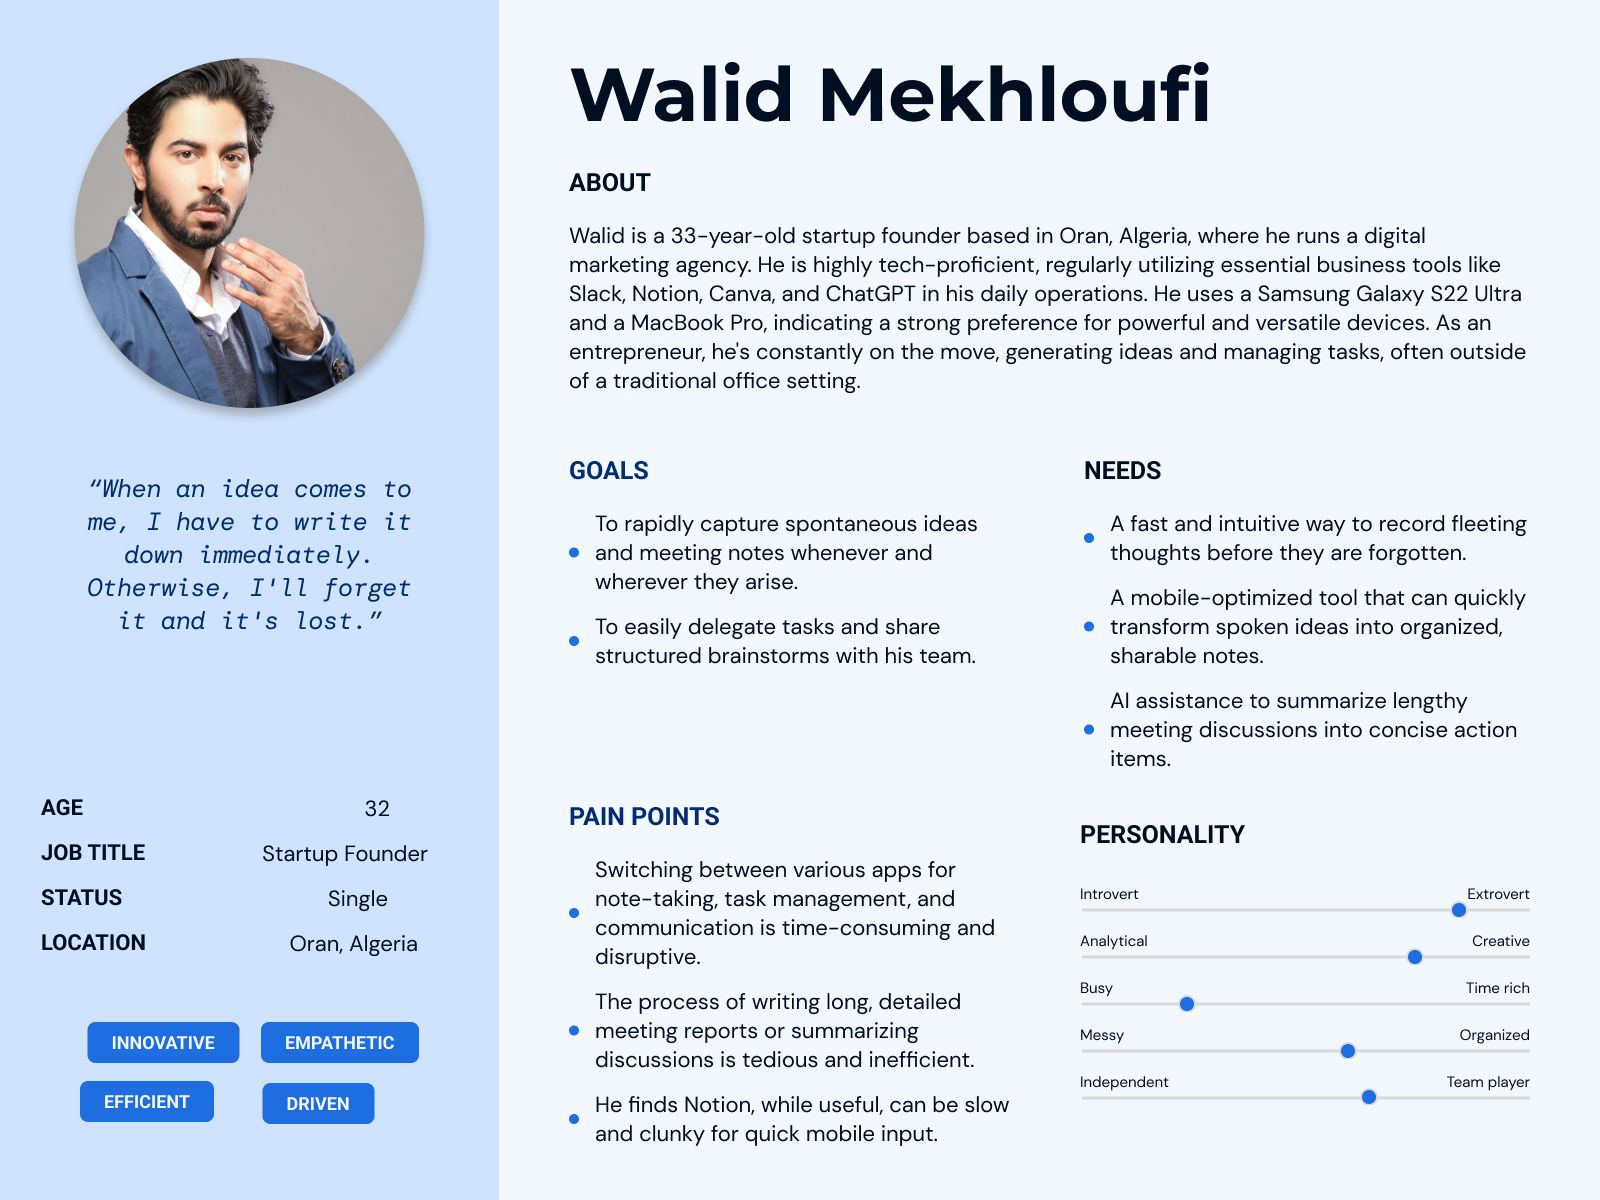
\includegraphics[width=\textwidth]{assets/docs/walid-persona.jpg}
    \end{figure}



    \paragraph{Persona 2: Walid l'Entrepreneur}

    \begin{itemize}
        \item \textbf{Profil:} Fondateur de startup de 33 ans (agence de marketing digital) à Oran. Il utilise des outils comme Slack, Notion, et ChatGPT sur son Samsung Galaxy S22 Ultra et MacBook Pro.
        \item \textbf{Objectifs:} Capturer rapidement les idées spontanées, déléguer facilement des tâches, et organiser ses idées et tâches par commandes vocales, notamment en déplacement.
        \item \textbf{Besoins:} Un moyen rapide pour enregistrer ses pensées, un outil mobile qui transforme la parole en notes structurées et partageables, et une IA pour résumer les réunions en actions concrètes.
        \item \textbf{Frustrations:} Oublie souvent des idées précieuses faute de pouvoir les noter instantanément, perd du temps à jongler entre les applications, et trouve la rédaction de comptes-rendus longue et inefficace.
        \item \textbf{Citation:} "Quand une idée me vient, je dois l’écrire direct. Sinon, je l’oublie et c’est mort."
    \end{itemize}
    
    
    % ===============================
    % Section: Wireframes et Design System
    % ===============================
    
    \subsection{Wireframes de l'application mobile}
    
    Avant le prototypage final, des wireframes basse fidélité ont été réalisés pour définir la structure et l'expérience utilisateur de l'application mobile SayNote.
    
    % Explication brève avant la figure
        \textit{La figure suivante présente un wireframe représentatif de l'application mobile.}
    \begin{figure}[H]
        \centering
        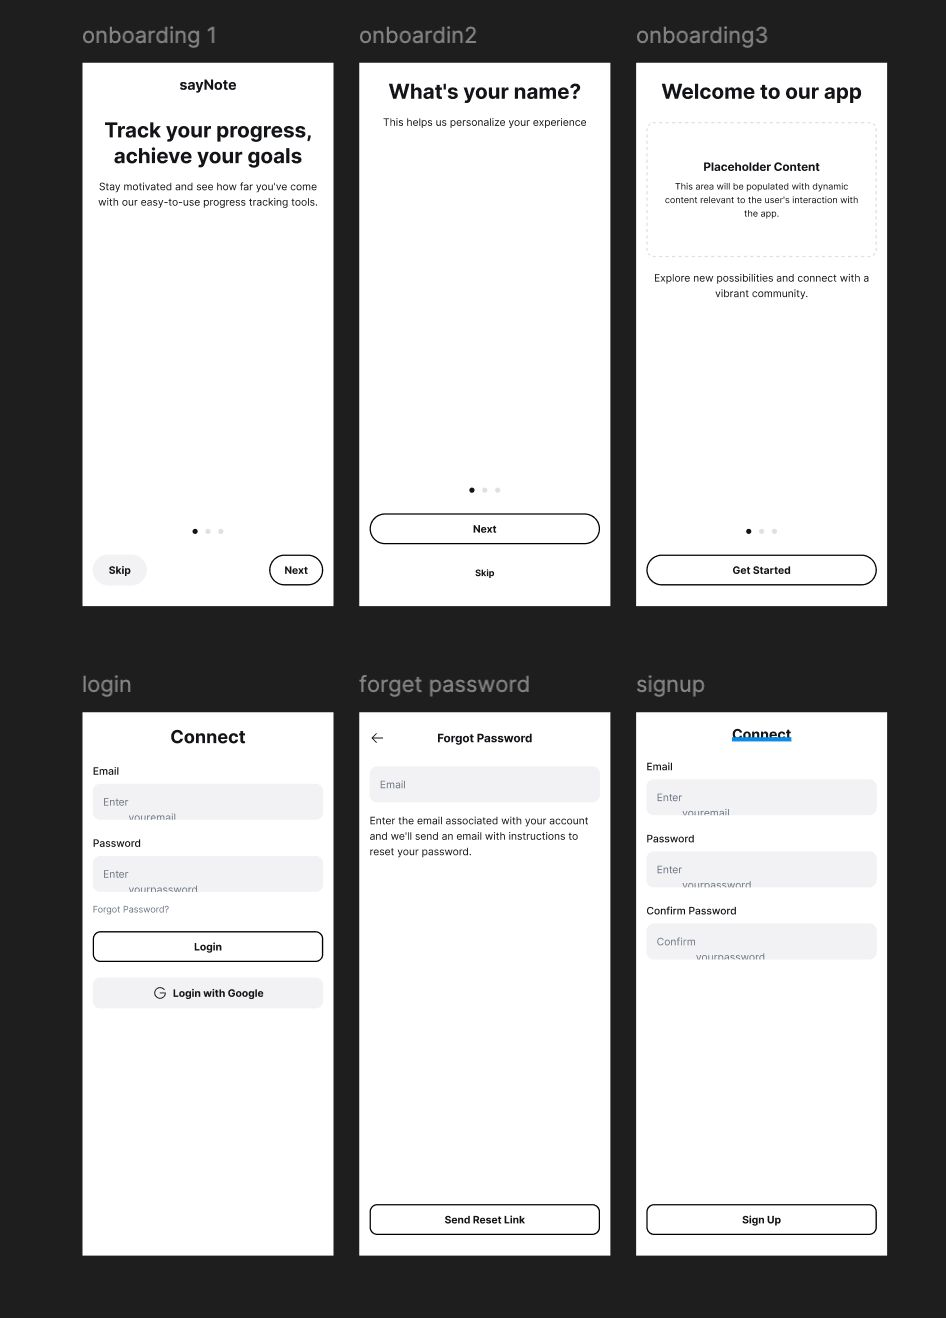
\includegraphics[width=0.9\textwidth]{assets/docs/mobile/wireframe_app-1.jpg}
        \caption{Wireframe de l'application mobile SayNote. \newline\textit{Ce schéma illustre la navigation et la disposition générale des écrans de authentification.}}
        \label{fig:wireframe_app_auth}
    \end{figure}
    
    \begin{figure}[H]
        \centering
        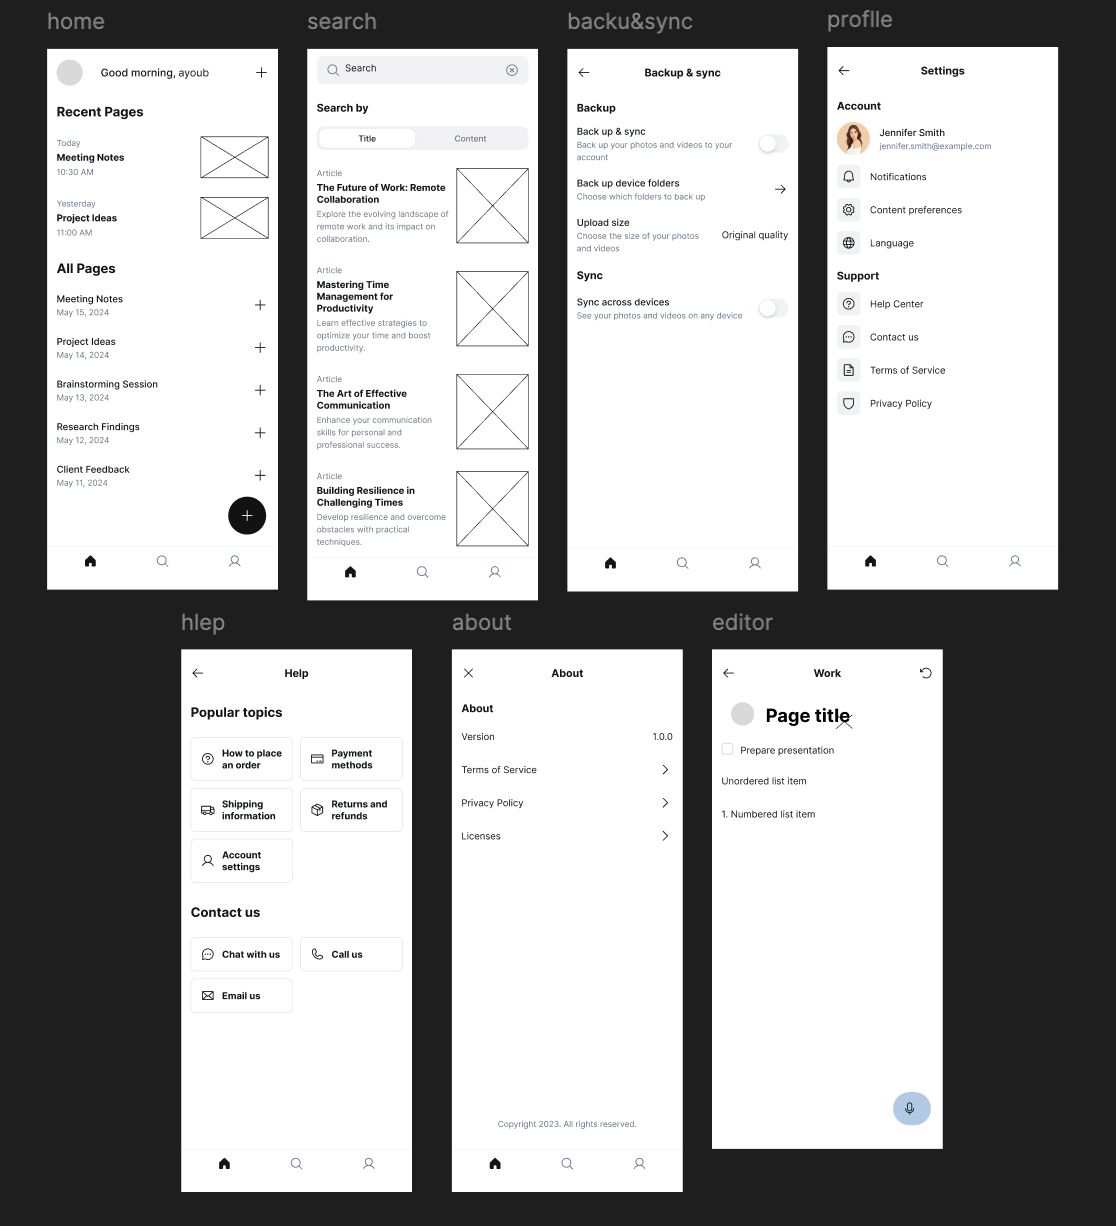
\includegraphics[width=0.9\textwidth]{assets/docs/mobile/wireframe_app-2.jpg}
        \caption{Wireframe de l'application mobile SayNote. \newline\textit{Ce schéma illustre la navigation et la disposition générale des écrans principaux.}}
        \label{fig:wireframe_app_main}
    \end{figure}
    
    
    \subsection{Synthèse du Design System}
    
    Une synthèse du design system a été réalisée pour garantir la cohérence visuelle et fonctionnelle de l'ensemble des interfaces.
    
        
    \subsubsection{Scénarios d'utilisations}
    
    Pour chaque persona, nous avons développé des scénarios d'utilisation qui illustrent comment SayNote répondrait à leurs besoins spécifiques:
    
    \paragraph{Scénario 1: Yasmine en cours d'Algorithmique}
    
    Yasmine est en cours d'algorithmique, une matière dense où les concepts s'enchaînent rapidement.
    \begin{enumerate}
        \item Elle lance SayNote et commence à enregistrer l'audio du cours tout en tapant les points clés.
        \item Quand le professeur aborde un nouveau chapitre, elle utilise la commande vocale "Nouveau titre: Complexité des algorithmes de tri" pour structurer sa note en temps réel.
        \item Elle dit "Ajouter bloc de code" pour insérer rapidement un exemple de pseudo-code que le professeur écrit au tableau.
        \item Plus tard, en révisant, elle utilise la commande "Résumer les points clés de cette section" pour obtenir une synthèse générée par IA, ce qui lui fait gagner du temps.
        \item Elle crée une sous-page "Exercices sur les tris" directement liée à sa note de cours pour centraliser sa théorie et sa pratique.
    \end{enumerate}
    
    \paragraph{Scénario 2: Walid a une idée de campagne en voiture}
    
    Walid est en voiture entre deux rendez-vous lorsqu'une idée de campagne marketing lui vient à l'esprit.
    \begin{enumerate}
        \item Il active SayNote en mode mains libres et dit "Nouvelle idée: Campagne de fin d'année pour le client Z".
        \item Il dicte les concepts clés de la campagne: l'audience cible, le message principal et les canaux de diffusion.
        \item Il utilise la commande "Créer une liste de tâches: Actions pour l'équipe marketing" pour lister les premières étapes.
        \item Il enchaîne avec "Assigner la tâche 'étude de la concurrence' à Sarah" pour déléguer une action immédiatement.
        \item Arrivé au bureau, il ouvre la note sur son MacBook, déjà structurée, et la partage sur le canal Slack de son équipe pour discussion.
    \end{enumerate}
    
    \section{Conception du système d'information}
    
    \subsection{Identification des acteurs}
    
    Le système SayNote interagit avec plusieurs types d'acteurs, chacun ayant des objectifs et des interactions spécifiques:
    
    \begin{itemize}
        \item \textbf{Utilisateur non authentifié:} Peut explorer la landing page, créer un compte ou se connecter.
        
        \item \textbf{Utilisateur authentifié:} Le principal acteur du système, qui peut créer, modifier, organiser et exporter des notes.
        
        \item \textbf{API Gemini:} Acteur système externe qui traite les commandes vocales et retourne des instructions structurées.
        
        \item \textbf{Service de stockage:} Acteur système responsable de la persistance et de la synchronisation des données.
    \end{itemize}
    
    \subsection{Diagramme de cas d'utilisation}
    
    Le diagramme de cas d'utilisation ci-dessous illustre les principales interactions entre les acteurs et le système SayNote:
    
    % Explication brève avant chaque figure
        \begin{figure}[htbp]
        \centering
        \includegraphics[width=0.9\textwidth]{assets/docs/SayNote_use_case.png}
        \caption{Diagramme de cas d'utilisation principal pour SayNote. \newline\textit{Ce diagramme UML met en évidence les interactions principales entre l'utilisateur et le système, servant de base à la conception fonctionnelle.}}
        \label{fig:use_case_diagram}
    \end{figure}
    
    Les principaux cas d'utilisation incluent:
    
    \begin{itemize}
        \item \textbf{Gestion du compte:} Inscription, connexion, modification du profil.
        
        \item \textbf{Gestion des notes:} Création, édition, suppression, création de sous-pages.
        
        \item \textbf{Interaction vocale:} Dictée de contenu, commandes de formatage, navigation par la voix.
        
        \item \textbf{Édition structurée:} Manipulation des blocs, formatage du texte, insertion d'éléments riches.
        
        \item \textbf{Recherche et filtrage:} Recherche textuelle, filtrage par date.
        
        \item \textbf{Exportation:} Export des notes vers différents formats.
    \end{itemize}
    
    \subsection{Diagrammes de séquence}
    
    Pour illustrer les interactions dynamiques entre l'utilisateur, l'application et les services externes, nous avons créé des diagrammes de séquence pour les processus clés.
    
    \subsubsection{Séquence de commande vocale}
    
    Le diagramme suivant montre la séquence d'interactions lors de l'utilisation d'une commande vocale pour manipuler le contenu:
    
    % Explication brève avant chaque figure
        \begin{figure}[htbp]
        \centering
        \includegraphics[width=0.85\textwidth]{assets/docs/SayNote_sequence_voice.png}
        \caption{Diagramme de séquence pour le traitement d'une commande vocale. \newline\textit{Ce diagramme UML détaille le déroulement des interactions lors de l'utilisation d'une commande vocale.}}
        \label{fig:sequence_voice_command}
    \end{figure}
    
    \subsubsection{Séquence de création et sauvegarde de note}
    
    Ce diagramme illustre le processus de création, d'édition et de sauvegarde d'une note:
    
    % Explication brève avant chaque figure
        \begin{figure}[htbp]
        \centering
        \includegraphics[width=0.85\textwidth]{assets/docs/SayNote_sequence_save.png}
        \caption{Diagramme de séquence pour la création et sauvegarde d'une note. \newline\textit{Ce diagramme UML montre le processus de création et de sauvegarde d'une note, mettant en évidence les interactions entre l'utilisateur et le système.}}
        \label{fig:sequence_save_note}
    \end{figure}
    
    \subsubsection{Séquence d'authentification}
    
    Ce diagramme illustre le processus d'authentification des utilisateurs dans l'application:
    
    % Explication brève avant chaque figure
        \begin{figure}[htbp]
        \centering
        \includegraphics[width=0.85\textwidth]{assets/docs/SayNote_auth_sequence.png}
        \caption{Diagramme de séquence pour l'authentification. \newline\textit{Ce diagramme UML explicite les étapes de vérification et de validation lors de la connexion d'un utilisateur.}}
        \label{fig:sequence_auth}
    \end{figure}
    
    \subsection{Diagrammes de base de données}
    
    \subsubsection{Diagramme entité-relation}
    
    Le modèle entité-relation ci-dessous représente la structure conceptuelle des données pour SayNote:
    
    % Explication brève avant chaque figure
        \begin{figure}[htbp]
        \centering
        \includegraphics[width=0.9\textwidth]{assets/docs/SayNote_er_diagram.png}
        \caption{Diagramme entité-relation pour SayNote. \newline\textit{Ce diagramme technique présente la structure conceptuelle de la base de données, essentielle pour la gestion des données.}}
        \label{fig:er_diagram}
    \end{figure}
    
    Les principales entités et leurs relations sont:
    
    \begin{itemize}
        \item \textbf{User:} Stocke les informations utilisateur (email, nom d'affichage, avatar).
        
        \item \textbf{Note:} L'entité centrale qui contient les métadonnées d'une note (titre, date de création/modification, propriétaire).
        
        \item \textbf{Block:} Représente un bloc individuel dans une note, avec son type, contenu et position.
        
        \item \textbf{Subpage:} Gère la relation hiérarchique entre les notes, permettant la création de sous-pages.
        
        \item \textbf{VoiceCommand:} Stocke les commandes vocales et leurs paramètres.
    \end{itemize}
    
    \subsubsection{Diagramme de base de données}
    
    Le schéma logique de la base de données traduit le modèle entité-relation en une structure implémentable:
    
    % Explication brève avant chaque figure
        \begin{figure}[htbp]
        \centering
        \includegraphics[width=0.9\textwidth]{assets/docs/SayNote_db_schema.png}
        \caption{Schéma logique de la base de données pour SayNote. \newline\textit{Ce schéma technique traduit le modèle conceptuel en tables relationnelles pour l'implémentation.}}
        \label{fig:db_schema}
    \end{figure}
    
    Notre implémentation utilise une base de données PostgreSQL hébergée sur Supabase, avec les tables principales suivantes:
    
    \begin{itemize}
        \item \textbf{users:} id, email, display\_name, avatar\_url, created\_at, updated\_at
        
        \item \textbf{notes:} id, title, user\_id, created\_at, updated\_at, is\_archived
        
        \item \textbf{blocks:} id, note\_id, parent\_block\_id, type, content, position, created\_at, updated\_at
        
        \item \textbf{subpages:} id, parent\_note\_id, child\_note\_id, position, created\_at
        
        \item \textbf{voice\_commands:} id, user\_id, command\_text, intent\_type, parameters, created\_at
    \end{itemize}
    
    \section{Conclusion}
    
    Ce chapitre a présenté notre approche méthodique de la planification du projet SayNote et de la conception de son expérience utilisateur. En combinant une méthodologie agile avec une approche de Design Thinking centrée sur l'utilisateur, nous avons établi un cadre solide pour le développement d'une application qui répond véritablement aux besoins des utilisateurs.
    
    La recherche utilisateur approfondie et l'élaboration de personas détaillés nous ont permis de comprendre intimement les défis et les aspirations de nos utilisateurs cibles. Les scénarios d'utilisation ont illustré comment SayNote s'intégrerait naturellement dans leurs flux de travail quotidiens, offrant une valeur réelle et des améliorations tangibles à leur expérience de prise de notes.
    
    La conception technique du système, illustrée par les diagrammes de cas d'utilisation, de séquence et de base de données, fournit une base solide pour l'implémentation qui sera détaillée dans le chapitre suivant. Cette architecture a été conçue pour être robuste, évolutive et flexible, permettant d'accommoder les futures améliorations et extensions de l'application.
    
    Les prochaines étapes consistent à transformer cette conception en un produit fonctionnel à travers le développement technique, en restant fidèle à notre vision d'une application de prise de notes révolutionnaire qui libère la créativité et la productivité de ses utilisateurs grâce à la puissance de la voix. 
    
    % --- Conclusion non numérotée ---
    \vspace{1cm}
    \begin{center}
    \textbf{\large Conclusion du Chapitre}
    \end{center}
    
        En résumé, ce chapitre a posé les bases méthodologiques et conceptuelles du projet SayNote. Il a mis en avant l'importance de la planification agile, de la recherche utilisateur, de la modélisation UML et de la conception technique pour garantir le succès de l'implémentation. Les éléments présentés ici serviront de référence pour le développement détaillé exposé dans le chapitre suivant.